\documentclass[11pt]{article}
\usepackage[margin=1in]{geometry}
\usepackage{amsmath,booktabs,array,xcolor,graphicx}
\usepackage[colorlinks=true,linkcolor=blue!50!black,urlcolor=blue!50!black]{hyperref}
\newcommand{\code}[1]{\texttt{\small #1}}
\setlength{\parskip}{4pt}\setlength{\parindent}{0pt}

\title{\vspace{-2em}TRADES Sampler Acceleration: Diagnosis \& State of Play}
\author{}\date{\vspace{-3em}}

\begin{document}
\maketitle\vspace{-2em}

An order moves the price only if it is \emph{marketable} (crosses the spread and executes). Depth
is decoded in \code{WorldAgent.py}$\to$\code{\_postprocess\_generated\_TRADES} as
\[
\text{depth} = \operatorname{round}(z_d\,\sigma_d + \mu_d), \quad \sigma_d=2.68,\ \mu_d=1.38,
\qquad\text{marketable}\iff \text{depth}<0 \iff z_d<-0.52 .
\]
Preprocessing \textbf{clamps depth $\ge 0$}, so the model is trained to pile depth at the best
quote (a spike). \emph{The marketable tail is thus a sampling artifact}: it appears only when
sampling noise spills the output below the boundary. Approximating the depth output as Gaussian
with std $s$, the marketable fraction is $\Phi(-0.52/s)$:
\begin{center}
\begin{tabular}{lccc}
\toprule
depth-output std $s$ & 1.0 (calibrated) & 0.5 & 0.3 (few-step deterministic)\\
marketable fraction & 30\% & 15\% & \textbf{4\% (frozen)}\\
\bottomrule
\end{tabular}
\end{center}

\textbf{Deterministic few-step sampling contracts $s$} onto the conditional mean $\Rightarrow$ spike
stays at 0 $\Rightarrow$ no executions $\Rightarrow$ passive orders build immovable walls
$\Rightarrow$ mid frozen. \textbf{DDPM works because its per-step noise is learned and load-bearing}
(\code{ddpm\_single\_step}, IDDPM variance $\log v = f\log\beta_t+(1-f)\log\tilde\beta_t$), keeping
$s$ near its trained value ($\sim$24\% marketable). \textbf{DDIM$(\eta{=}1)\neq$ DDPM}: in
\code{ddim\_single\_step} the noise scale is the fixed lower bound $\eta\sqrt{\tilde\beta_t}$, so it
under-samples the tail. \textbf{Many-step deterministic DDIM diverges} (stiff probability-flow ODE
on an under-trained score field: conditioning reaches $+265\sigma$, price crashes 34\%).

\section{What we tried (all flag-gated, default off)}

\begin{center}
\begin{tabular}{p{6.2cm} p{2.2cm} p{6.0cm}}
\toprule
Hypothesis / fix & Flag & Outcome\\
\midrule
Type-decode geometry biases order type & \code{--type-decode prior} & Fixes $\eta{=}1$ market-order blow-up + drift; does \emph{not} unfreeze\\
Conditioning time channel frozen & \code{--fix-time} & No effect; drove time channel OOD\\
Cancels dropped w/o exact match & \code{--fix-cancel-bind} & No effect on freeze\\
LOB padding inverted vs training & \code{--fix-lob-pad} & No effect (book rarely thin)\\
Type-2 cancels in conditioning & \code{--drop-type2-cond} & Marginal\\
Order-flow imbalance builds walls & order TTL & Caused mass-cancel hang; reverted; no fix\\
OOD price conditioning ($-5.7\sigma$) & mid-rel.\ norm & Reverted; DDPM fine despite it\\
Restore tail via depth temperature & \code{--depth-temp $\kappa$} & \textbf{Cliff, not a dial} (\S3)\\
Tail is set in early high-noise steps & \code{HYBRID\_DDPM\_PP} & \textbf{Confirmed} (\S3)\\
\bottomrule
\end{tabular}
\end{center}

\section{Key results}

\textbf{(a) Stochasticity must be early.} Same checkpoint / 10 NFE, only \emph{placement} of noise
differs (\code{gaussian\_diffusion.py} hybrids): DDPM-head $+$ ODE-tail moves (113 mids); the inverse
(ODE head $+$ DDPM tail) stays frozen (5 mids). The marketable tail is decided in the high-noise
steps; a stochastic \emph{tail} cannot recover it.

\textbf{(b) Depth-temperature is a switch, not a dial.} $\kappa$ multiplies $z_d$, but the collapsed
output is a \emph{spike} (72\% at depth 0) sitting on the boundary, so $\kappa$ slides it across
wholesale:
\begin{center}
\begin{tabular}{lccccc}
\toprule
$\kappa$ & 1.0 & 1.5 & 2.0 & 3.0 & target (real / DDPM)\\
marketable \% & 2 & 55 & 54 & 52 & $\sim$3 / $\sim$24\\
unique mids & 6 & 193 & 164 & 191 & 69 / 23\\
price drift & \$0.02 & \$2.0 & \$4.5 & \$7.9 & $\sim$\$0.4 / \$0.1\\
\bottomrule
\end{tabular}
\end{center}
No intermediate $\kappa$ hits the target; a scalar cannot peel a 3\% tail off a spike --- the
distribution must come from the model.

\textbf{(c) Deterministic samplers are hypersensitive to checkpoint calibration; DDPM is robust.}
\begin{center}
\begin{tabular}{lcc}
\toprule
checkpoint & DDIM$_{10}\ \eta{=}0$ & DDPM$_{100}$\\
\midrule
val 0.681 (tighter conditional) & \textbf{frozen} (6 mids, 0\% mkt) & works ($\sim$24\% mkt)\\
val 0.719 (broader conditional) & \textbf{explodes} (109 mids, 36\% mkt, $+$\$1.3) & works ($\sim$24\% mkt)\\
\bottomrule
\end{tabular}
\end{center}
The two checkpoints behave \emph{oppositely} under deterministic DDIM; DDPM's noise dominates and
washes out the miscalibration. Validation loss went the \emph{wrong} way ($0.681\!\to\!0.719$ as
training progressed) --- so \textbf{val loss is not a valid model selector} here.

\section{Cross-check with the paper (arXiv:2502.07071)}

Main results and the released \code{TRADES-LOB} dataset use \textbf{DDPM, 100 steps}; we confirmed by
analysing their INTC file (depth std 2.02, 3.1\% marketable, moving market --- DDPM-quality), and
now use it as our realism benchmark. Single-step DDIM is disclosed as a lossy $100\times$
acceleration (predictive score $1.213\!\to\!3.146$). We verified from \code{ddim\_single\_step} that
at one step the model contributes \textbf{$\sim$1.7\%} of the output ($\bar\alpha_1{=}0.998$, near
clean): it is a \emph{near-marginal regime}, not a graceful accelerator --- the disclosed score
collapse is the fingerprint of that.

\section{Figures: order-flow \& market-order composition}

\begin{figure}[htbp]\centering
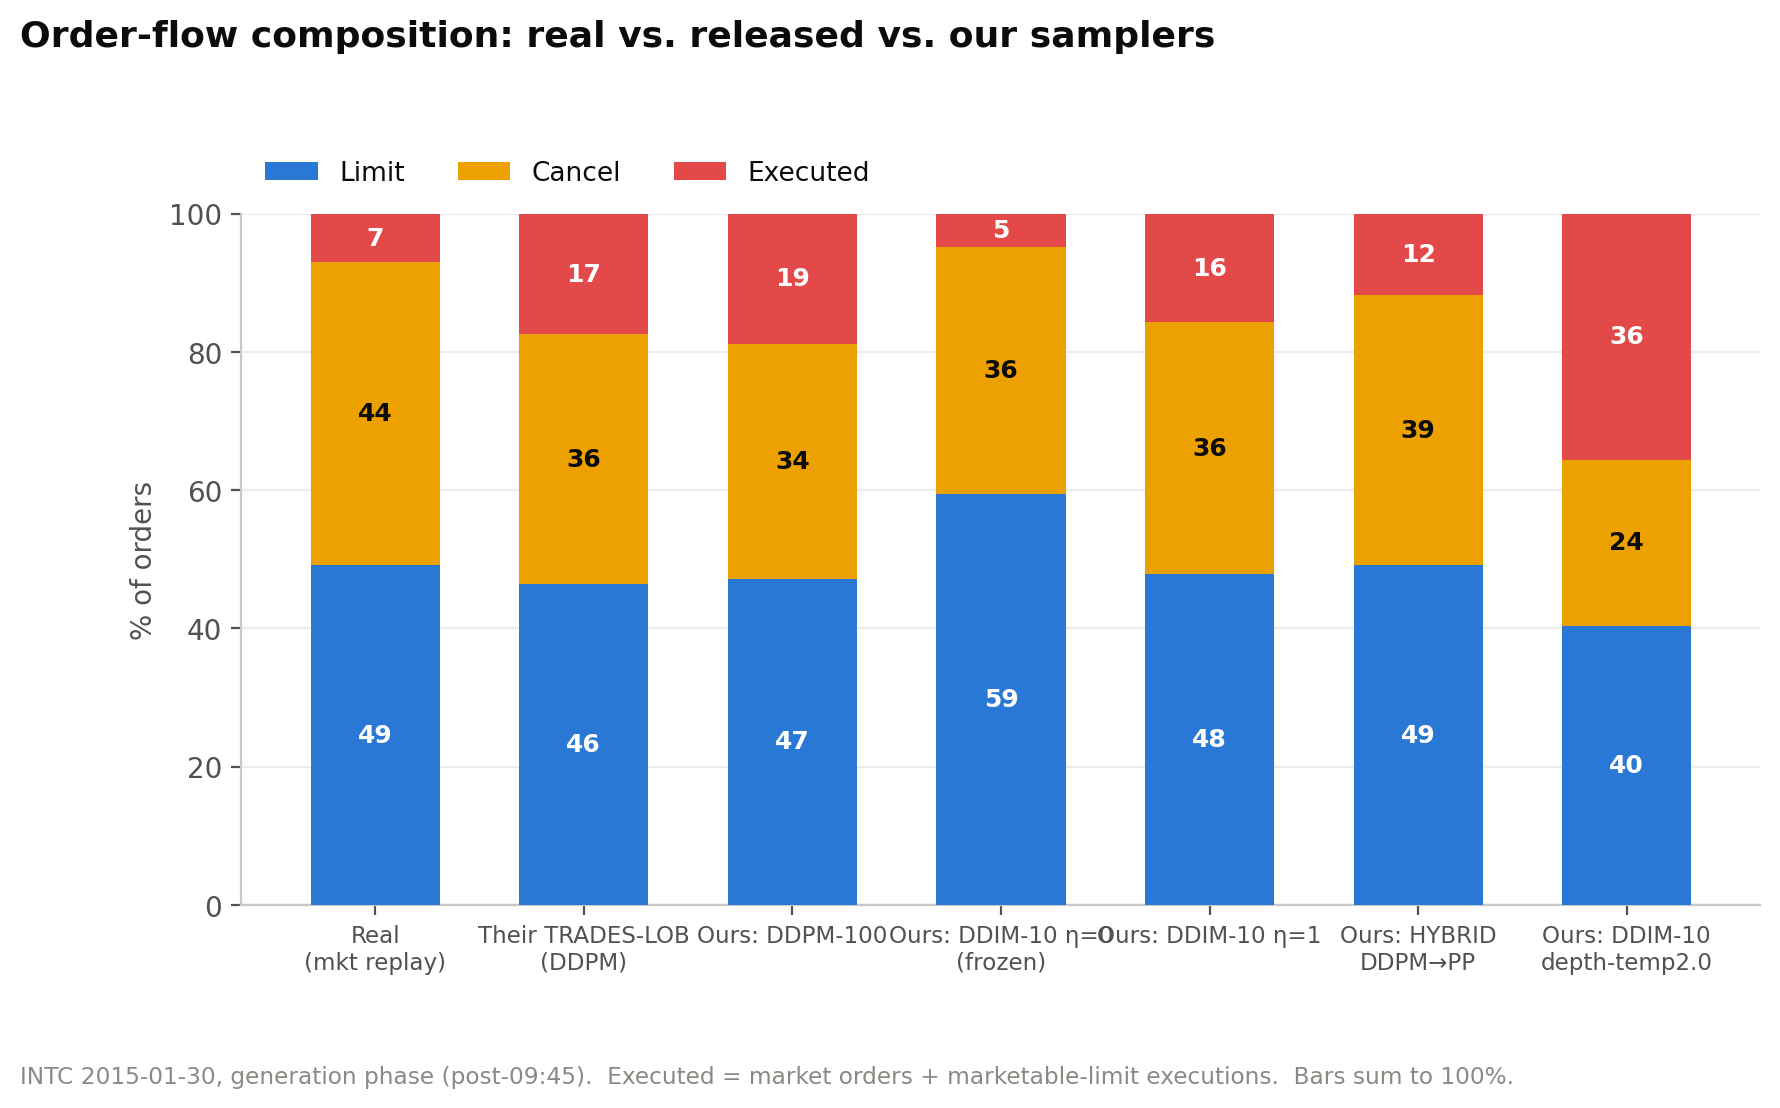
\includegraphics[width=0.9\linewidth]{figures/flow_mix_comparison.png}
\caption{Order-type composition (limit/cancel/executed), measured identically in the real
market-replay, the authors' released \code{TRADES-LOB} (DDPM), and our runs. Even the released
gold-standard \emph{over-executes} (17\% vs real 7\%); frozen DDIM under-executes (5\%); depth-temp
over-executes badly (36\%). ``Executed'' bundles market orders and marketable-limit executions and
cannot be split from the output CSV.}
\end{figure}

\begin{figure}[htbp]\centering
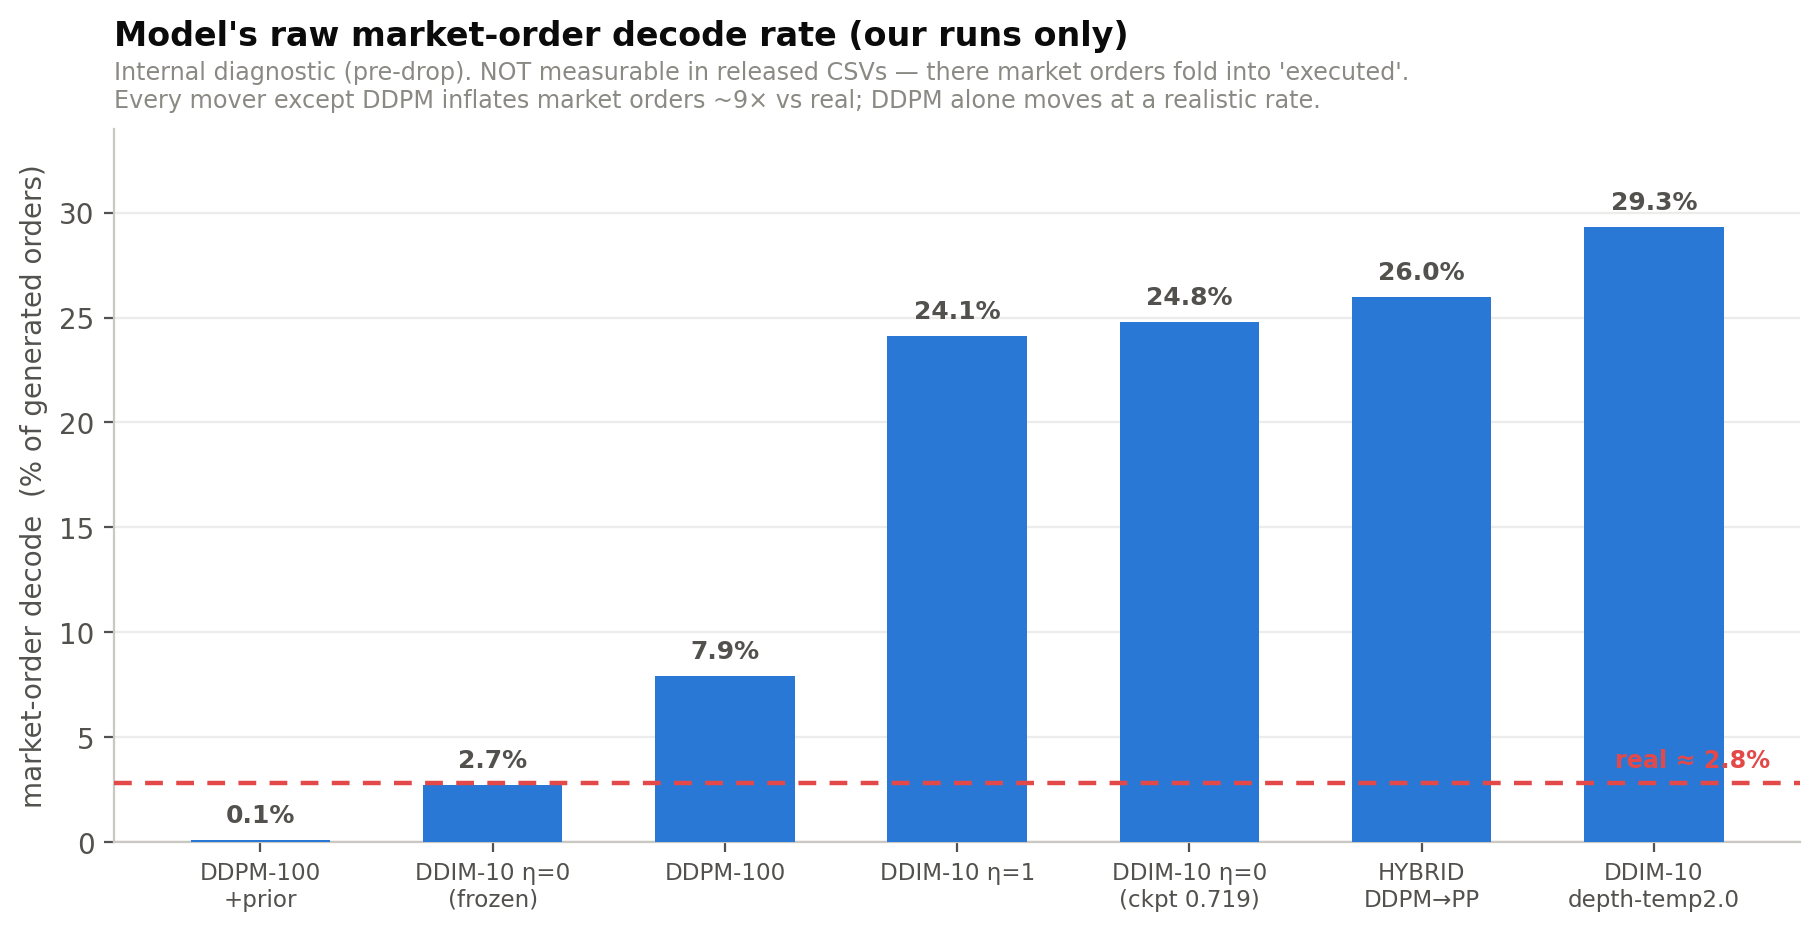
\includegraphics[width=0.9\linewidth]{figures/market_decode_rate.png}
\caption{The model's raw \emph{market-order decode} rate --- our internal pre-drop diagnostic,
\emph{not} measurable in any released CSV (there market orders fold into ``executed''). DDPM is the
only sampler that moves the market at a realistic rate ($\sim$8\%); every other configuration that
produces movement inflates market orders to $\sim$25--29\% ($\approx$9$\times$ real) --- the drift
mechanism.}
\end{figure}

\begin{table}[htbp]\centering\small
\textbf{(a) Flow composition} --- measurable in all CSVs\\[2pt]
\begin{tabular}{lccc}
\toprule
source & Limit \% & Cancel \% & Exec \%\\
\midrule
Real (market replay) & 49.2 & 43.8 & 7.0\\
Their \code{TRADES-LOB}, INTC 30 (DDPM) & 46.4 & 36.2 & 17.3\\
Their \code{TRADES-LOB} (INTC/TSLA, 29--30) & 45.9--46.6 & 36.2--39.4 & 14.0--17.3\\
Ours: DDPM-100 & 47.2 & 34.0 & 18.8\\
Ours: DDIM-10 $\eta{=}0$ (frozen) & 59.4 & 35.8 & 4.8\\
Ours: DDIM-10 $\eta{=}1$ & 47.8 & 36.5 & 15.7\\
Ours: HYBRID DDPM$\to$PP (8+2) & 49.1 & 39.1 & 11.8\\
Ours: DDIM-10 depth-temp 2.0 & 40.4 & 24.0 & 35.7\\
\bottomrule
\end{tabular}

\vspace{8pt}
\textbf{(b) Market-order decode \%} --- our runs only (real $\approx$2.8\%; not measurable in released CSVs)\\[2pt]
\begin{tabular}{lc@{\hspace{2em}}lc}
\toprule
run & mkt \% & run & mkt \%\\
\midrule
DDPM-100 + prior & 0.08 & DDIM-10 $\eta{=}1$ & 24.1\\
DDIM-10 $\eta{=}0$ (frozen) & 2.7 & DDIM-10 $\eta{=}0$ (ckpt 0.719) & 24.8\\
DDPM-100 & 7.9 & HYBRID DDPM$\to$PP (8+2) & 26.0\\
 & & DDIM-10 depth-temp 2.0 & 29.3\\
\bottomrule
\end{tabular}
\end{table}

\section{State of play \& next steps}

\textbf{Established:} DDPM works and replicates their benchmark (base model sound); deterministic
fast samplers fail via depth-variance collapse; stochasticity is load-bearing and must be injected
early; a decode-time scalar cannot reconstruct the tail; deterministic behaviour is set by
checkpoint calibration, not val loss.

\textbf{In progress:} retraining with \code{CONDITIONAL\_DROPOUT=0.1} --- targets a better-calibrated
conditional and activates the unused classifier-free-guidance path
(\code{\_forward\_with\_guidance}, \code{--guidance-scale}).

\textbf{Open:} does a well-calibrated checkpoint let moderate-step deterministic / hybrid sampling
hold the DDPM benchmark at a fraction of the cost? Can guidance tune realism / market impact? Then:
downstream execution-agent training in the accelerated simulator.

\textbf{Contributions:} (1) faithful accelerated closed-loop LOB sampling requires stochasticity ---
deterministic ODE solvers collapse the marketable-order tail; (2) deterministic samplers are
hypersensitive to conditional-variance calibration where stochastic ones are robust (val loss
invalid as selector); (3) single-step DDIM is a degenerate near-marginal regime, quantified.

\end{document}
